% Options for packages loaded elsewhere
\PassOptionsToPackage{unicode}{hyperref}
\PassOptionsToPackage{hyphens}{url}
\PassOptionsToPackage{dvipsnames,svgnames,x11names}{xcolor}
%
\documentclass[
  11pt,
]{article}

\usepackage{amsmath,amssymb}
\usepackage{iftex}
\ifPDFTeX
  \usepackage[T1]{fontenc}
  \usepackage[utf8]{inputenc}
  \usepackage{textcomp} % provide euro and other symbols
\else % if luatex or xetex
  \usepackage{unicode-math}
  \defaultfontfeatures{Scale=MatchLowercase}
  \defaultfontfeatures[\rmfamily]{Ligatures=TeX,Scale=1}
\fi
\usepackage{lmodern}
\ifPDFTeX\else  
    % xetex/luatex font selection
\fi
% Use upquote if available, for straight quotes in verbatim environments
\IfFileExists{upquote.sty}{\usepackage{upquote}}{}
\IfFileExists{microtype.sty}{% use microtype if available
  \usepackage[]{microtype}
  \UseMicrotypeSet[protrusion]{basicmath} % disable protrusion for tt fonts
}{}
\makeatletter
\@ifundefined{KOMAClassName}{% if non-KOMA class
  \IfFileExists{parskip.sty}{%
    \usepackage{parskip}
  }{% else
    \setlength{\parindent}{0pt}
    \setlength{\parskip}{6pt plus 2pt minus 1pt}}
}{% if KOMA class
  \KOMAoptions{parskip=half}}
\makeatother
\usepackage{xcolor}
\usepackage[left=2.54cm,right=2.54cm]{geometry}
\setlength{\emergencystretch}{3em} % prevent overfull lines
\setcounter{secnumdepth}{5}
% Make \paragraph and \subparagraph free-standing
\makeatletter
\ifx\paragraph\undefined\else
  \let\oldparagraph\paragraph
  \renewcommand{\paragraph}{
    \@ifstar
      \xxxParagraphStar
      \xxxParagraphNoStar
  }
  \newcommand{\xxxParagraphStar}[1]{\oldparagraph*{#1}\mbox{}}
  \newcommand{\xxxParagraphNoStar}[1]{\oldparagraph{#1}\mbox{}}
\fi
\ifx\subparagraph\undefined\else
  \let\oldsubparagraph\subparagraph
  \renewcommand{\subparagraph}{
    \@ifstar
      \xxxSubParagraphStar
      \xxxSubParagraphNoStar
  }
  \newcommand{\xxxSubParagraphStar}[1]{\oldsubparagraph*{#1}\mbox{}}
  \newcommand{\xxxSubParagraphNoStar}[1]{\oldsubparagraph{#1}\mbox{}}
\fi
\makeatother


\providecommand{\tightlist}{%
  \setlength{\itemsep}{0pt}\setlength{\parskip}{0pt}}\usepackage{longtable,booktabs,array}
\usepackage{calc} % for calculating minipage widths
% Correct order of tables after \paragraph or \subparagraph
\usepackage{etoolbox}
\makeatletter
\patchcmd\longtable{\par}{\if@noskipsec\mbox{}\fi\par}{}{}
\makeatother
% Allow footnotes in longtable head/foot
\IfFileExists{footnotehyper.sty}{\usepackage{footnotehyper}}{\usepackage{footnote}}
\makesavenoteenv{longtable}
\usepackage{graphicx}
\makeatletter
\def\maxwidth{\ifdim\Gin@nat@width>\linewidth\linewidth\else\Gin@nat@width\fi}
\def\maxheight{\ifdim\Gin@nat@height>\textheight\textheight\else\Gin@nat@height\fi}
\makeatother
% Scale images if necessary, so that they will not overflow the page
% margins by default, and it is still possible to overwrite the defaults
% using explicit options in \includegraphics[width, height, ...]{}
\setkeys{Gin}{width=\maxwidth,height=\maxheight,keepaspectratio}
% Set default figure placement to htbp
\makeatletter
\def\fps@figure{htbp}
\makeatother
% definitions for citeproc citations
\NewDocumentCommand\citeproctext{}{}
\NewDocumentCommand\citeproc{mm}{%
  \begingroup\def\citeproctext{#2}\cite{#1}\endgroup}
\makeatletter
 % allow citations to break across lines
 \let\@cite@ofmt\@firstofone
 % avoid brackets around text for \cite:
 \def\@biblabel#1{}
 \def\@cite#1#2{{#1\if@tempswa , #2\fi}}
\makeatother
\newlength{\cslhangindent}
\setlength{\cslhangindent}{1.5em}
\newlength{\csllabelwidth}
\setlength{\csllabelwidth}{3em}
\newenvironment{CSLReferences}[2] % #1 hanging-indent, #2 entry-spacing
 {\begin{list}{}{%
  \setlength{\itemindent}{0pt}
  \setlength{\leftmargin}{0pt}
  \setlength{\parsep}{0pt}
  % turn on hanging indent if param 1 is 1
  \ifodd #1
   \setlength{\leftmargin}{\cslhangindent}
   \setlength{\itemindent}{-1\cslhangindent}
  \fi
  % set entry spacing
  \setlength{\itemsep}{#2\baselineskip}}}
 {\end{list}}
\usepackage{calc}
\newcommand{\CSLBlock}[1]{\hfill\break\parbox[t]{\linewidth}{\strut\ignorespaces#1\strut}}
\newcommand{\CSLLeftMargin}[1]{\parbox[t]{\csllabelwidth}{\strut#1\strut}}
\newcommand{\CSLRightInline}[1]{\parbox[t]{\linewidth - \csllabelwidth}{\strut#1\strut}}
\newcommand{\CSLIndent}[1]{\hspace{\cslhangindent}#1}

\usepackage[noblocks]{authblk}
\renewcommand*{\Authsep}{, }
\renewcommand*{\Authand}{, }
\renewcommand*{\Authands}{, }
\renewcommand\Affilfont{\small}
\usepackage{lipsum} \usepackage{libertine}
\makeatletter
\@ifpackageloaded{caption}{}{\usepackage{caption}}
\AtBeginDocument{%
\ifdefined\contentsname
  \renewcommand*\contentsname{Table of contents}
\else
  \newcommand\contentsname{Table of contents}
\fi
\ifdefined\listfigurename
  \renewcommand*\listfigurename{List of Figures}
\else
  \newcommand\listfigurename{List of Figures}
\fi
\ifdefined\listtablename
  \renewcommand*\listtablename{List of Tables}
\else
  \newcommand\listtablename{List of Tables}
\fi
\ifdefined\figurename
  \renewcommand*\figurename{\textbf{Fig.}}
\else
  \newcommand\figurename{\textbf{Fig.}}
\fi
\ifdefined\tablename
  \renewcommand*\tablename{Table}
\else
  \newcommand\tablename{Table}
\fi
}
\@ifpackageloaded{float}{}{\usepackage{float}}
\floatstyle{ruled}
\@ifundefined{c@chapter}{\newfloat{codelisting}{h}{lop}}{\newfloat{codelisting}{h}{lop}[chapter]}
\floatname{codelisting}{Listing}
\newcommand*\listoflistings{\listof{codelisting}{List of Listings}}
\makeatother
\makeatletter
\makeatother
\makeatletter
\@ifpackageloaded{caption}{}{\usepackage{caption}}
\@ifpackageloaded{subcaption}{}{\usepackage{subcaption}}
\makeatother

\ifLuaTeX
  \usepackage{selnolig}  % disable illegal ligatures
\fi
\usepackage{bookmark}

\IfFileExists{xurl.sty}{\usepackage{xurl}}{} % add URL line breaks if available
\urlstyle{same} % disable monospaced font for URLs
\hypersetup{
  pdftitle={Producing population-level estimates of internal displacement in Ukraine using GPS mobile phone data},
  pdfauthor={Rodgers Iradukunda; Francisco Rowe; Elisabetta Pietrostefani},
  colorlinks=true,
  linkcolor={blue},
  filecolor={Maroon},
  citecolor={Blue},
  urlcolor={Blue},
  pdfcreator={LaTeX via pandoc}}


\title{\textbf{Producing population-level estimates of internal
displacement in Ukraine using GPS mobile phone data}}


\author[1]{Rodgers Iradukunda}
\author[1]{Francisco Rowe}
\author[1]{Elisabetta Pietrostefani}

\affil[1]{Geographic Data Science Lab, Department of Geography and
Planning, University of Liverpool, Liverpool, United Kingdom}


\date{}
\begin{document}
\maketitle
\begin{abstract}
Nearly 110 million people are forcibly displaced people worldwide.
However, estimating the scale and patterns of internally displaced
persons in real time, and developing appropriate policy responses,
remain hindered by traditional data streams. They are infrequently
updated, costly and slow. Mobile phone location data can overcome these
limitations, but only represent a population segment. Drawing on an
anonymised large-scale, high-frequency dataset of locations from 25
million mobile devices, we propose an approach to leverage mobile phone
data and produce population-level estimates of internal displacement. We
use this approach to quantify the extent, pace and geographic patterns
of internal displacement in Ukraine during the early stages of the
Russian invasion in 2022. Our results produce reliable population-level
estimates, enabling real-time monitoring of internal displacement at
detailed spatio-temporal resolutions. Accurate estimations are crucial
to support timely and effective humanitarian and disaster management
responses, prioritising resources where they are most needed.
\end{abstract}


\newpage

The forced displacement of individuals, including refugees,
asylum-seekers and internally displaced people (IDP), creates
considerable humanitarian, social and economic
costs\textsuperscript{1,2}. Recent estimates indicates that the number
of forcibly displaced populations has significantly grown as result of
persecution, conflict, violence, human rights violations and
disasters\textsuperscript{3}. As of June 2023, the United Nations High
Commissioner for Refugees (UNHCR) estimated 110 million of forcibly
displaced people worldwide, with the number of IDP (62.5 million)
accounting for the largest share of these
displacements\textsuperscript{4}. The Russian full-scale invasion of
Ukraine is estimated to have created the fastest global displacement
crisis, and one of the largest, since the Second World
War\textsuperscript{2}.

Forcibly displaced population data are key to inform operational plans,
humanitarian responses and long-term policy making. By understanding the
scale and locations where people are forcibly fleeing and the extent of
their return, government agencies, aid organisations and local community
groups can better prioritise and allocate resources and services where
they are most needed in the required quantities\textsuperscript{3}.
Highly granular geographical data tracking population displacements in
real time are therefore critical to support these
efforts\textsuperscript{5,6}.

Traditional data systems are constrained to render information at such
high temporal and geographical resolution and speed. Over the years,
UNHCR and the Internal Displacement Monitoring Centre (IDMC) have made
significant efforts triangulating various data sources to improve and
deliver global databases that enable the monitoring and management of
forced population displacements\textsuperscript{3}. However, they have
also identified persistent challenges in the production of reliable
estimates of forcibly displaced
populations\textsuperscript{7,8}.Traditional data systems are not
regularly updated, costly and characterised by slow data collection and
release\textsuperscript{9}. Particularly in conflict areas, humanitarian
partners and data collectors often face access restrictions due to
violence and insecurity preventing data gathering\textsuperscript{4}.
Data streams may also have gaps collecting data on displacement during
short-term evacuations or spontaneous movements resulting from conflict
and violence\textsuperscript{10,11}. The danger and challenging nature
of field work in conflict zones can also disrupt continuous engagement
in data collection by humanitarian and development
agencies\textsuperscript{12,13}.

Novel digital footprint data have emerged as a key source of information
offering an opportunity to capture human population movements at highly
granular geographical and temporal scales\textsuperscript{9,14}.These
data are automatically and continuously generated avoiding exposure of
data collectors to hazardous areas and minimising potential data
gaps\textsuperscript{10}. Mobile phone location data have increasingly
been used to monitor population movements during crises, particularly
measuring exposure to ambient pollutant exposure\textsuperscript{16},
transport patterns\textsuperscript{17}, recreational
behaviour\textsuperscript{18}, disaster-induced displacement
(e.g.~flooding and earthquakes)\textsuperscript{19} and the spread of
diseases - notably during the COVID-19 pandemic\textsuperscript{20}.
Yet, limited work has been undertaken to estimate the scale and patterns
of IDP using mobile phone data. Additionally, differences in the access
and use of mobile phone technology and applications used to collect
location data prevent the production of reliable population-level
mobility estimates. Most existing work based on mobile phone data has
thus constrained to offer rough signals about population movements
(e.g.~spatial concentration), trends (e.g.~increasing) and changes
(e.g.~low to high)\textsuperscript{9}.

To address these gaps, we propose an approach to produce high-frequency
population-level estimates of internal displacement drawing on location
data from 25 million unique devices. Our first contribution is
methodological and illustrates how high-frequency footprint data can
enable the generation of population-level estimates of internal
displacement correcting for differences in mobile phone-derived and
actual population counts, moving beyond providing rough signals. Most
prior work leveraging on digital footprint data to estimate population
displacement relies on social media or call detail records, with
location being inferred resulting in reduced
precision\textsuperscript{21--23}. We use data collected via GPS
technology which provides greater precision data on
location\textsuperscript{24}.

Our second contribution is to provide evidence of the scale and spatial
patterns of population displacement in Ukraine during the first year of
the invasion. The Russian full-scale invasion of Ukraine has created the
fastest global displacement crisis, and one of the largest, since the
Second World War\textsuperscript{2}. Recent estimates suggest that
nearly one-third of Ukrainian residents are estimated to have been
forced from their homes\textsuperscript{2}. As of 25 September 2023,
3.67 million people were estimated to have been displaced internally
within Ukrainian borders\textsuperscript{25}. These estimates are based
on a random digit dial telephone survey aiming at generating a
nationally representative sample of 2,000 individuals at each monthly
round\textsuperscript{25}. While consistent with high frequency
estimates based on Facebook data\textsuperscript{26}, these estimates
cannot deliver population-level estimates of population displacement for
geographical areas, or high-temporal frequency. Our approach offers high
frequency population displacement estimates to complement data derived
from traditional data streams.

\section{Results}\label{results}

\subsection{Estimating the extent of internal population
displacement}\label{estimating-the-extent-of-internal-population-displacement}

We first estimate the extent of daily internal population displacement
at the oblast and raion level (Fig.~\ref{fig-popdisplacement}). We
estimate that over 5 million people were internally displaced from their
oblast of residence by April 2022 reaching an average of about 10
million in late July and August 2022. Fig.~\ref{fig-popdisplacement}
reveals a drop in population displacement during mid-June and mid-July,
coinciding with a pattern of return displacements primarily to the
cities of Kiev and Kharkhiv (see Section~\ref{sec-return}). In addition
to return movements, subsequently higher but fluctuating levels of
movement after mid July seem to reflect the shifting dynamics of the
armed conflict towards southeastern Ukraine where ware fire intensified
during this period\textsuperscript{27}.

\begin{figure}[h]

\begin{minipage}{\linewidth}

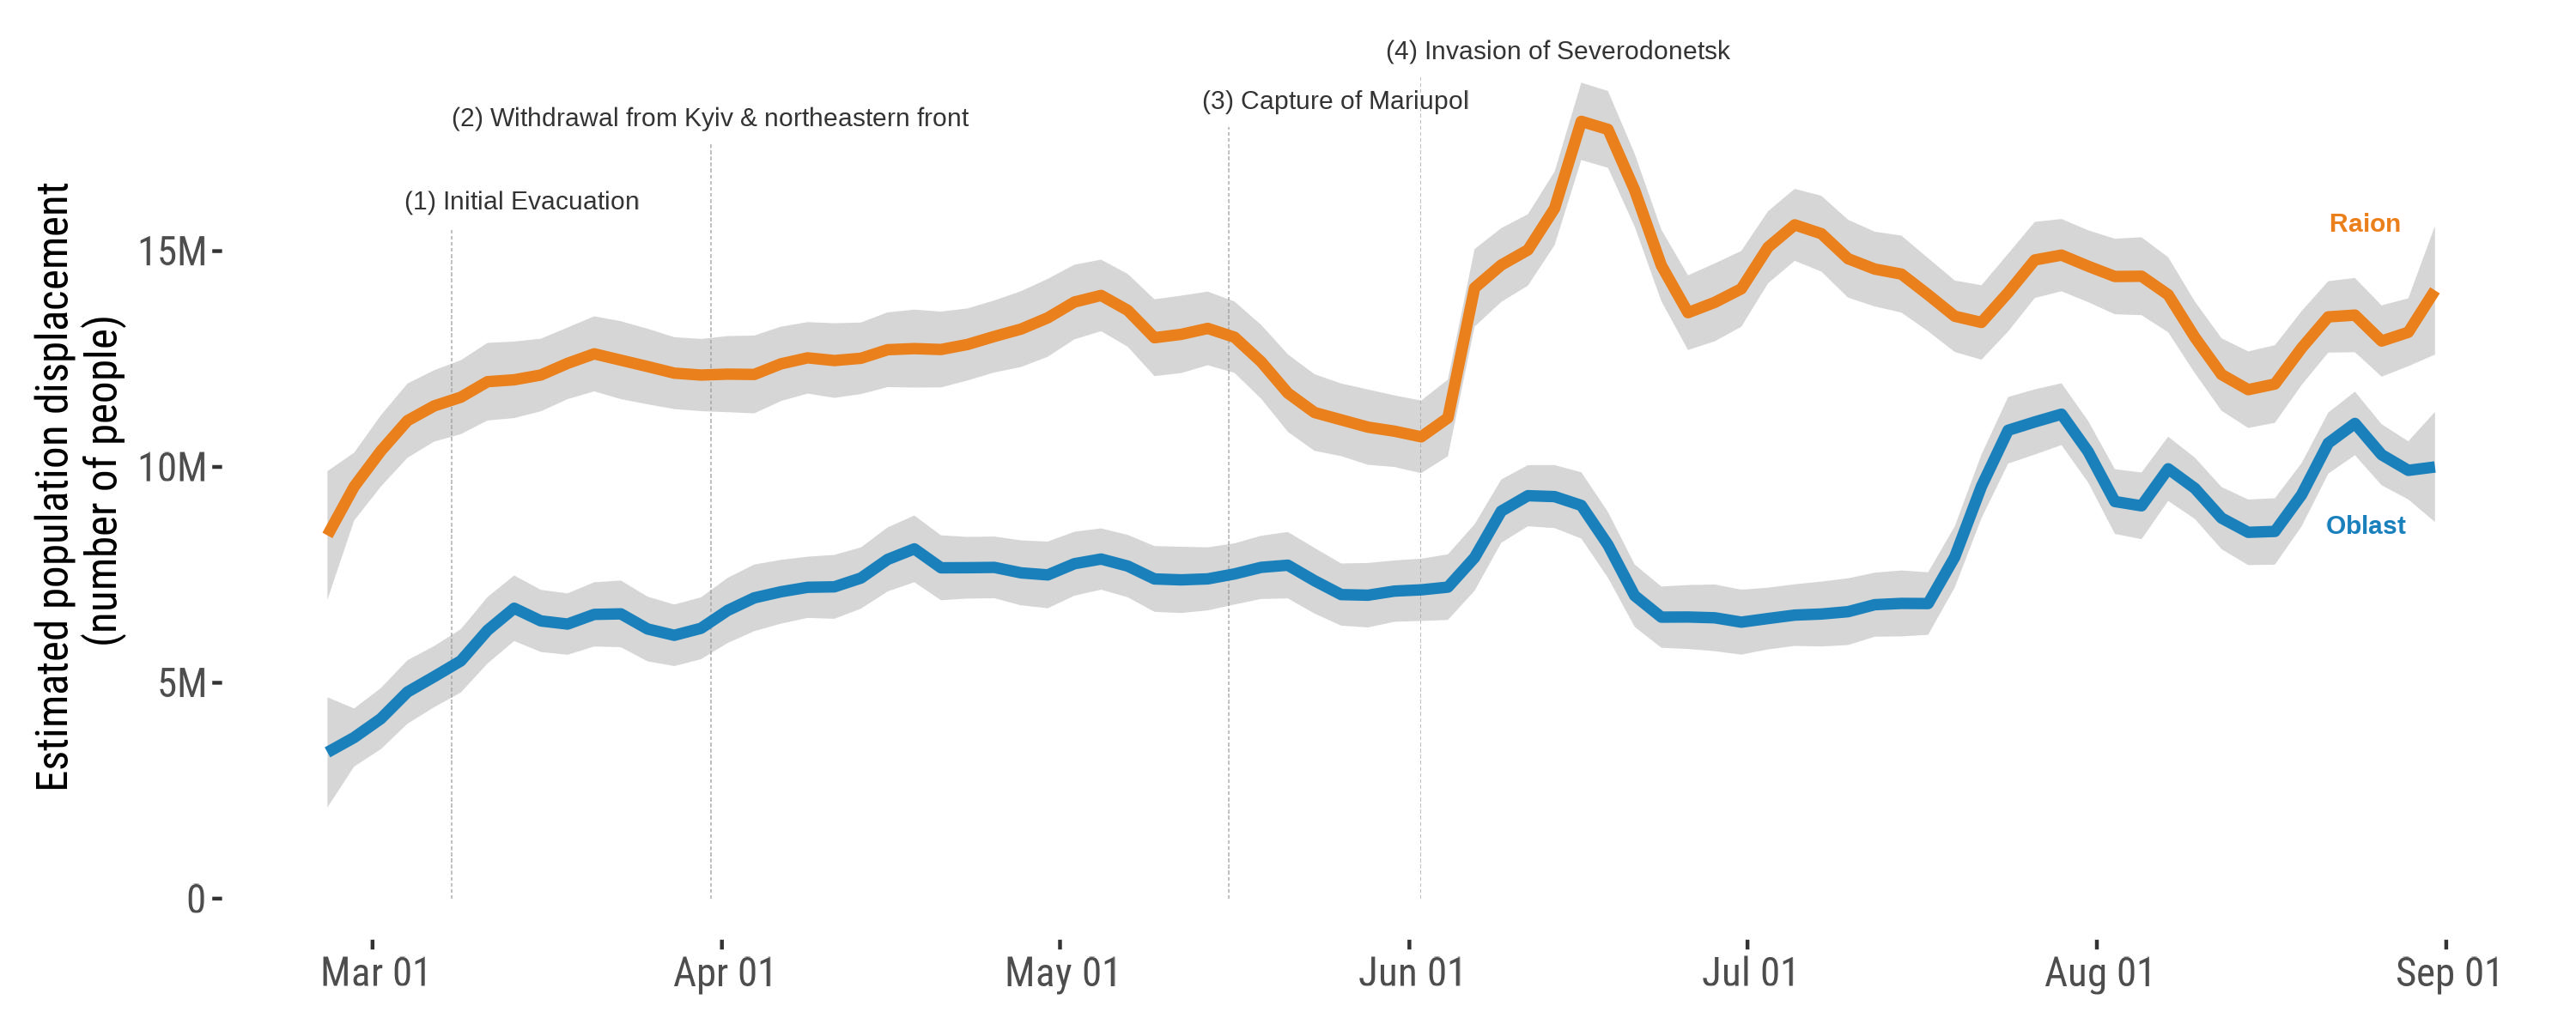
\includegraphics{../outputs/2_1/fig1.jpg}

\end{minipage}%

\caption{\label{fig-popdisplacement}\textbf{Estimated daily number of
displaced population. February to August 2022.} The number of displaced
people is estimated as the difference between the population in a region
for a given day after the start of the war and the population before the
war in 2020 - see Section~\ref{sec-methods2.2}.}

\end{figure}%

Our contribution is to generate geographically granular estimates of
internal displacement at the raion level leveraging the high spatial
precision of GPS data. As anticipated, the levels of raion-level
displacement consistently exceeds those of oblast-level displament as
they reflect movements that cannot be captured at higher levels of
spatial aggregation: raions within the same oblast's boundaries
capturing the fact that most displacement tend to occur over short
distances. Our raion-level estimates indicate a rise and peak of over 17
million displaced people in mid June 2022 following the start of the
Russian invasion of Severodonetsk. Around 90\% of the buildings and
infrastructure is estimated to have been destroyed or damaged after the
capture of Severodonetsk\textsuperscript{28}. From mid July, our
estimates indicate a rise in population displacement at the oblast
level, but such increase is not reflect at the raion level, indicating
that the most displacement that took place during this time tended to
occur over long distances involving a cross of oblast boundaries (see
Fig. S1 in Supplementary Material (SM) displaying distance
distributions).

Our findings are consistent with existing estimates. We compare our
oblast-level displacement estimates with existing estimates derived from
an United Nations - International Organization for Migration (IOM)
survey\textsuperscript{25} and Facebook data\textsuperscript{26} (see
Section~\ref{sec-methods2.2}, Tab. S1 and Fig. S2 in SM). The shape of
the temporal evolution of population displacement is remarkably
consistent. Though, we identify some discrepancies. Our estimates tend
to be higher than those produced by Leasure et al.~by approximately 250
thousand people across the time series. The difference can be explained
by Leasure et al.'s estimates are affected by power outages in the
Donetsk and Luhansk regions resulting in zero or small numbers for
various dates\textsuperscript{26,29} (see Fig. S3 in SM). Similarly, our
oblast-level estimates are noticable greater than the IOM figures in
June and August. We assume that this is because our estimates include
data from Crimea, and there was significant movement from and to Crimea
to Russian-occupied Ukrainian territory and Russia during these
months\textsuperscript{27}. This is as Russia started a ``volunteer
mobilisation'' and deployed new troops and logistics to support an a
frontline extending from Zaporizhzhia to Kherson, along the Dnieper
River\textsuperscript{27}. If we exclude Crimea, our estimates are much
closer to IOM and Leasure et al.'s estimates (see Tab. S1 in
\href{https://github.com/fcorowe/ukraine-pop-displacement/blob/main/manuscript/quarto-file-supplementary.pdf}{SM}).

\subsection{Identifying the main origins and
destinations}\label{sec-odm}

We then examine the net balance of internal population displacements
resulting inflows minus outflows, to identify the main areas losing and
gaining population through these displacements. As expected,
Fig.~\ref{fig-heatmaps}a reveals that Kiev City was the main area losing
population at the start of the war between late February and early May
before recording large positive net balances of over 2 million people.
These gains seem to echo large-scale return population movements as
Russian troops withdrew from the outskirts of Kiev City and focused on
the eastern and southern regions of Ukraine, particularly Donetsk,
Kharkiv, Crimea and Luhansk (Fig.~\ref{fig-heatmaps}b). Reflecting the
geographic concentration of military ground forces, these frontline
eastern and southern regions registered a consistent pattern of
population losses between March and August. Population losses are
particularly prominent in Donetsk where the estimated losses exceeded 2
million people in late July and early August 2022. To a lesser extent,
Odessa also displays a negative albeit moderate balance of population
displacements during the early months of the invasion as Russia had a
naval blockade on Ukrainian ports.

\begin{figure}[h]

\begin{minipage}{\linewidth}

\includegraphics[width=\textwidth,height=0.5\textheight]{../outputs/2_2/fig2_paper.pdf}

\end{minipage}%

\caption{\label{fig-heatmaps}\textbf{Net migration count by oblast and
raions, February to August 2022.} \textbf{a.} Weekly median net
migration by oblast. \textbf{b.} Monthly median net migration across
raions. \textbf{c.} Top ten raions with the largest cumulative net
negative (in blue) and positive (in red) migration balance organised
from the largest to the smallest. \textbf{d.} Changes in the share of
estimated population across the urban-rural hierarchy.}

\end{figure}%

At the same time, Fig.~\ref{fig-heatmaps}a reveals that western, central
and central-south areas tended to gain population during the early
months of the invasion between February and June 2022. These areas
include oblasts close to the border with Poland, Slovakia, Hungary,
Romania and Moldova, such as Ivano-Frankivs'k, Vinnytsya, Volyn and
Zakarpattia probably serving as transit centres for international
crossings and humanitarian assistance. Kirovohrad also shows
considerable positive population balances over the early months of the
war, most likely receiving population from frontline areas in eastern
parts of Ukraine. Fig.~\ref{fig-heatmaps}a shows that most of these
areas have tended to experience population losses as Kiev City and
Odessa record positive population balances from late July.

These aggregate patterns of population displacement conceal the local
concentration of net population losses and gains across raions.
Fig.~\ref{fig-heatmaps}c reports the net balance of population
displacements over time for the ten raions with the largest cumulative
losses and gains between February and August 2022. It reveals that
Kharkiv remained the raion with the largest cumulative loss of
population since the start of the war at least until August 2022, but it
reported positive balances as Ukrainian forces launched a
counteroffensive and liberated major settlements in the Kharkiv oblast
in late July and August 2022. The oblast of Donest'k seems to congregate
the raions with the greatest population losses, reflecting the
concentration of frontline activity in raions, such as Donets'ka,
Mariupol's'ka and Makivs'ka.

On the other hand, Fig.~\ref{fig-heatmaps}c reveals that raions within
the oblasts of Dnipropetrovsk, Kiev City and Donetsk recorded the
largest cumulative net migration gains at times when these oblasts
recorded moderate overall net migration losses
(Fig.~\ref{fig-heatmaps}a). The raions of Dniprodzerzhyns'ka,
Zhotovods'ka and Nikopol's'ka all registered large cumulative population
gains through net migration from February to August 2022 despite
systematic moderate overall negative migration balances in the oblast of
Dnipropetrovs'k. Similarly, the raion of lasynuvats'ka in Donestk
recorded a large cumulative net migration gain despite this being the
oblast with the largest negative migration balances. These results
suggest that people tended to move locally to neighbouring areas, or
were unable to afford moving to more distant locations in western
Ukraine (see Fig. S1).

Additionally, mapping the patterns of net migration
(Fig.~\ref{fig-heatmaps}b and Fig.~\ref{fig-heatmaps}d) reveals the
increasing prevalence of population loss through net migration in
Ukraine, particularly in less populated areas. In early weeks of the
invasion in February, negative net migration balances concentrated in
urban centres, especially Kiev and Khakiv. As the conflict evolved, net
migration losses seem to have expanded to most of the country
prominently reducing the relative national share of population in very
low density and low density rural areas (Fig.~\ref{fig-heatmaps}d).
These reductions in sparsely populous areas appear to have been mirrored
by a growing national share of population in urban centres, with Kiev
and Odessa acting as the major centres of population attraction in
August (Fig.~\ref{fig-heatmaps}d).

\subsection{Return movements}\label{sec-return}

Understanding the scale and pace of return movement to residential areas
in conflict zones after a period of displacement is also important to
shape and support humanitarian assistance, successful reintegration,
mental health and community rebuilding programmes\textsuperscript{30}.
Understanding return movements enables more efficient resource
allocation prioritising areas for infrastructure reconstruction and
service delivery\textsuperscript{30}. IOM estimated that 6 million
people had returned to their usual place of residence in Ukraine by
August 23 2022 following a two-week period elsewhere in the
country\textsuperscript{4}. At the time of writing, the most recent IOM
estimate puts this figure at 4.7 million returnees in April 11 2024,
14.2 per cent of whom returned from abroad\textsuperscript{31}. These
estimates are derived from a survey of 20 thousand people, with
follow-ups to 1,638 individuals identified as
returnees\textsuperscript{31}. The proportion of returnees for each
oblast is computed and multiplied by the total population in Ukraine to
derive return estimates. Returnees are identified as those respondents
who spent a two-week period away from their place of residence.

\begin{figure}[h]

\begin{minipage}{\linewidth}

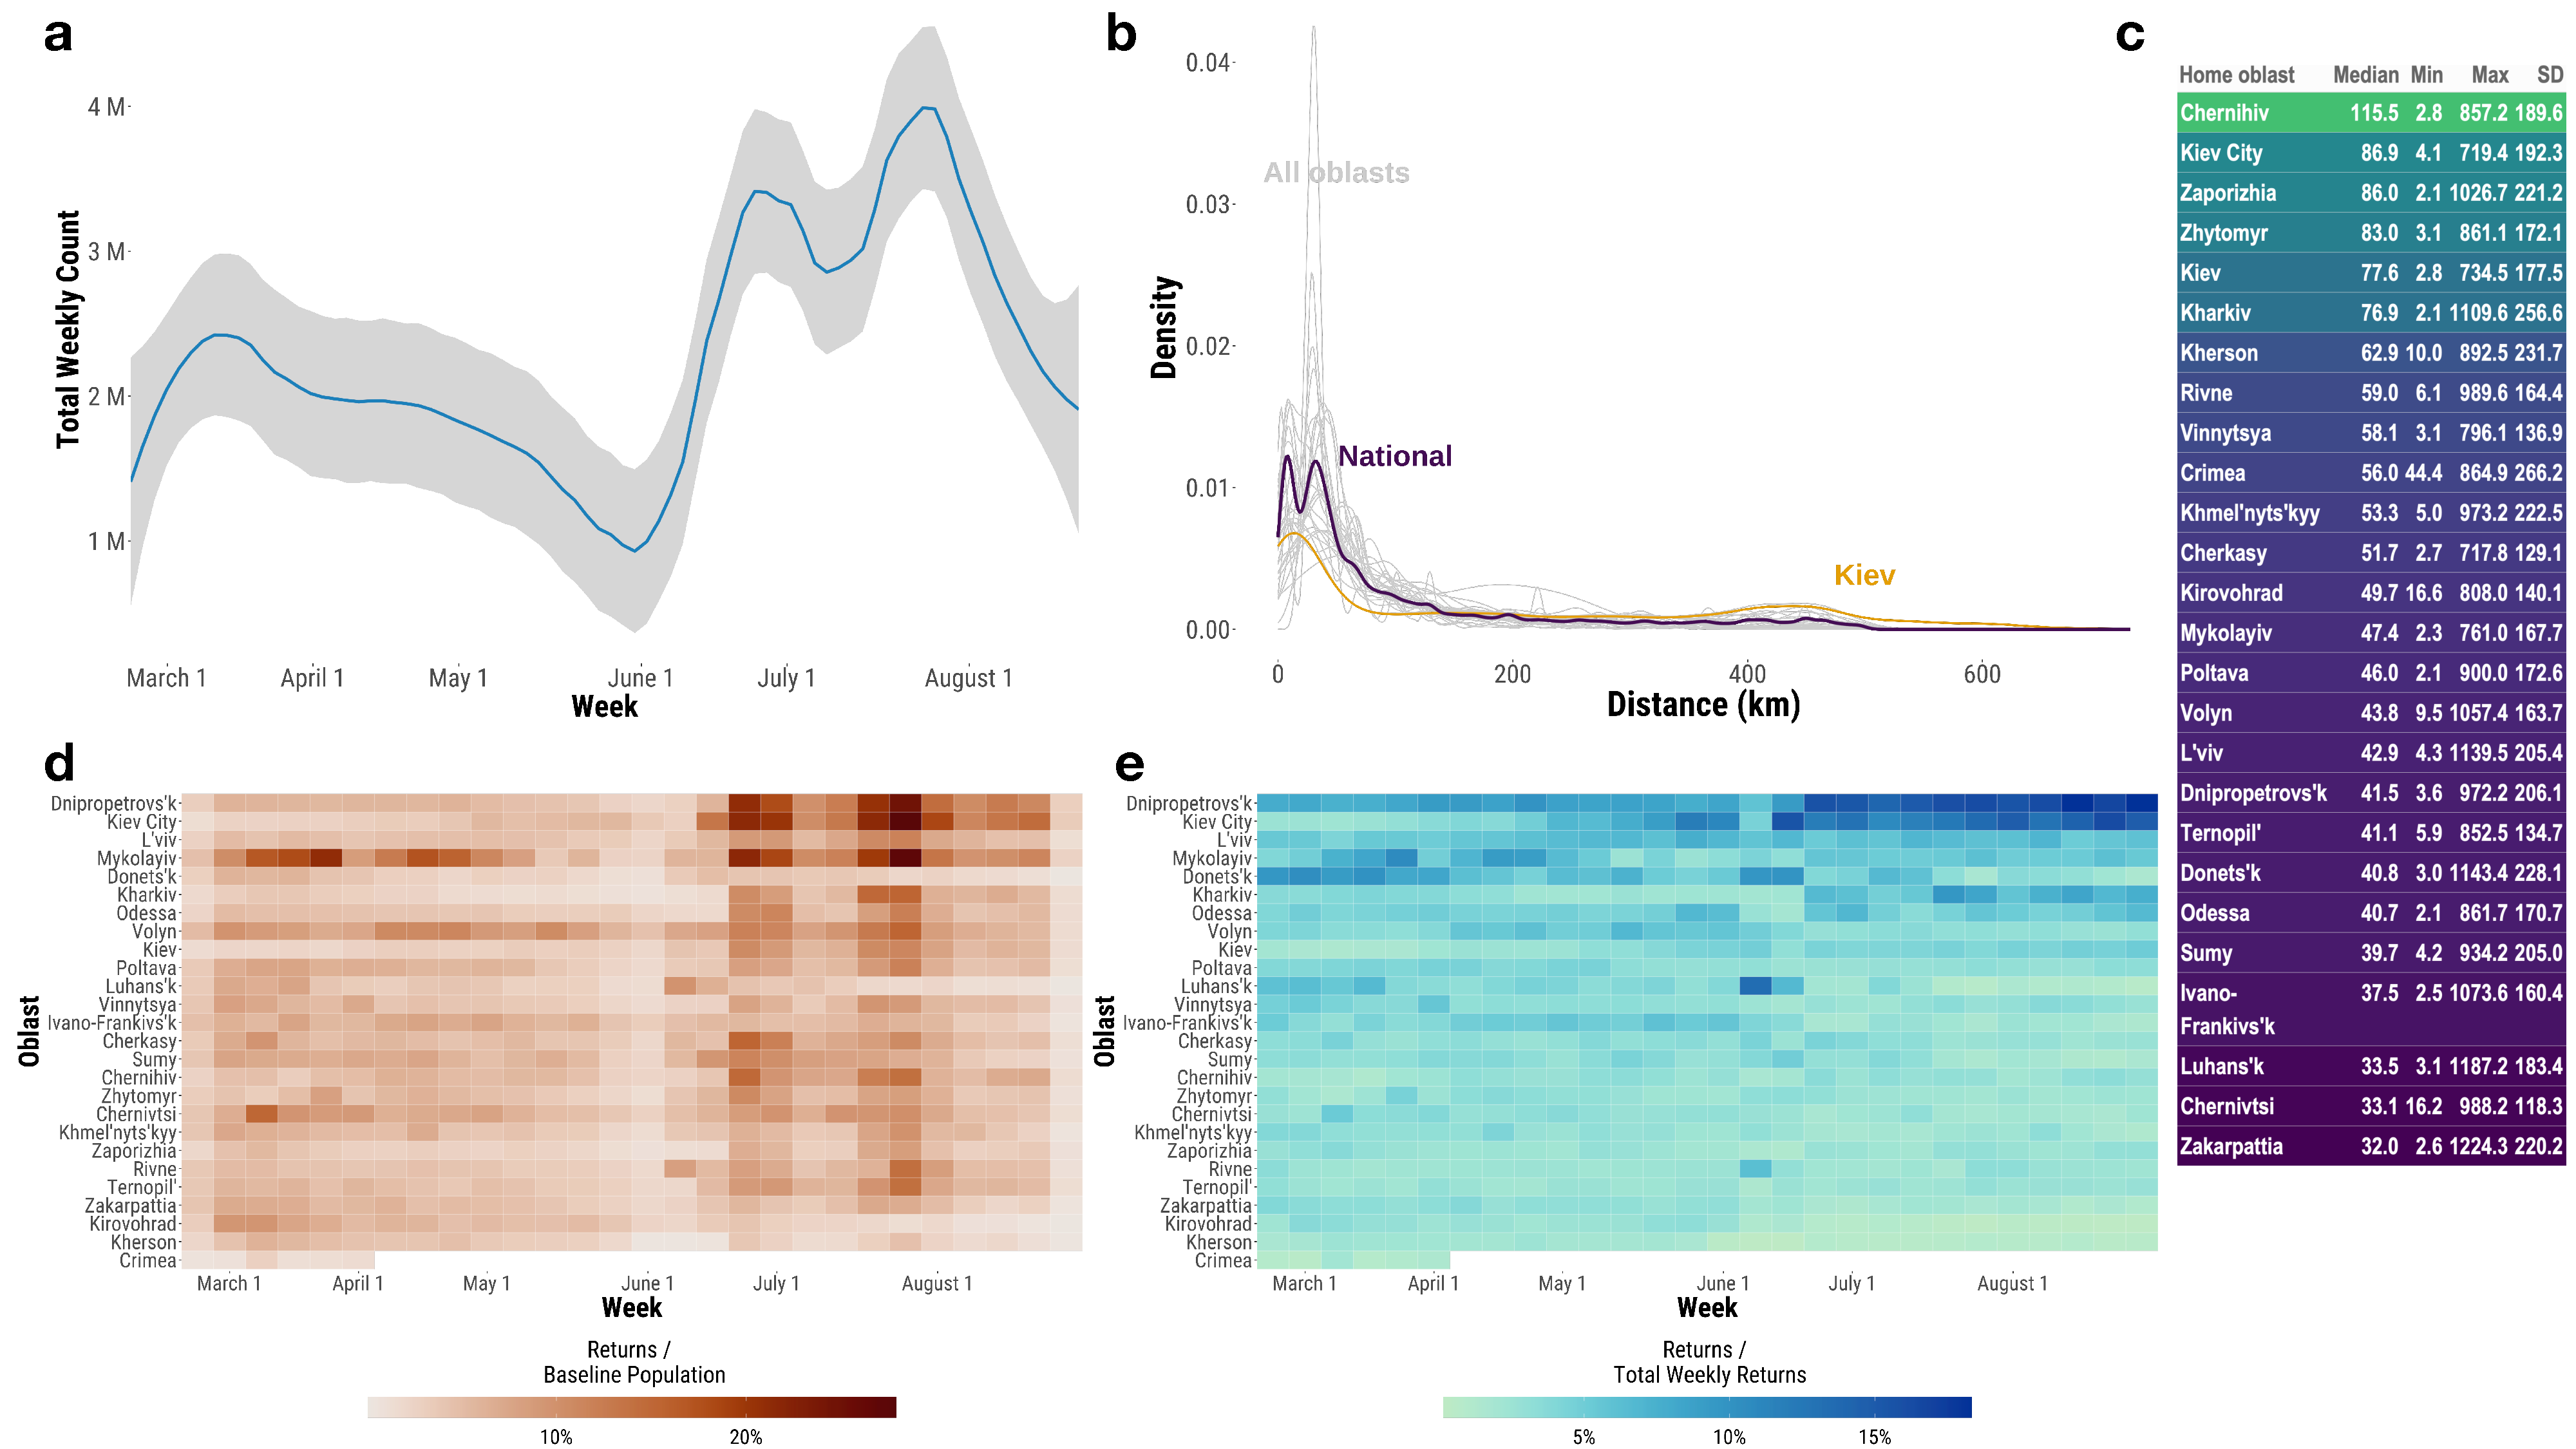
\includegraphics[width=\textwidth,height=0.5\textheight]{../outputs/2_3/dougs_returns/fig3.pdf}

\end{minipage}%

\caption{\label{fig-returns}\textbf{Return movements, February to August
2022.} \textbf{a.} Weekly total number of returns. Local polynomial
regression modelling was used to build 95\% confidence intervals.
\textbf{b.} Distribution of distance truncated to display return
movements below 700km. \textbf{c.} Median, minimum (min), maximum (max)
and standard deviation (SD) distance in km, oblast. \textbf{d.} Per cent
of returns over the total baseline population for individual oblasts
before the start of the war. \textbf{e.} Per cent of returns over the
total number of returns for individual oblasts.}

\end{figure}%

Using our methodology (see Section~\ref{sec-methods2.2}), we generate
estimates and expand this evidence providing information on the spatial
patterns, distance and pace of return movements
(Fig.~\ref{fig-returns}a-e). Our estimates indicate that just over 2
million people had returned to their place of residence before February
24 during the week commencing August 22, 2022 (Fig.~\ref{fig-returns}a).
Our estimates also showed considerable fluctuations over time,
reflecting that some of displacements and returns may be temporary. Some
people may return to their home location after spending a short period
of time elsewhere. Some may return to check on close relatives and
friends, examine local livability and recover belongings, and then
leave. The fluctuations observed in our estimates also reflect the fact
that we are unable to follow the same mobile phone devices for the
entire period of analysis. We observe some individual returns to the
same location, but are unable to identify their location in subsequent
periods. Crimea is a good example as we could only identify returns
until the first week of April but not thereafter
(Fig.~\ref{fig-returns}d-e).

Fig.~\ref{fig-returns}d-e reveal a differentiated rate of return
movements across oblasts. Dnipropetrovs'k and Kiev City display higher
proportions of return movements relative to their populations before the
start of the armed conflict, and to the total weekly number of returns
across Ukraine. L'viv and Mykolaiv record high rates of return movement
likely reflecting their role as transit points, food, temporary shelter
and accommodation centres for refugees, IDP and
troops\textsuperscript{32}. Kherson and Crimea register the lowest
number of returns. As indicated above, no returns were recorded for
Crimea after April 2022, and Kherson remained under Russian occupation
during our period of analysis.

Return movements tend to occur over relatively short distances
(Fig.~\ref{fig-returns}b-c). The median distance of return moves between
oblasts is less than 100km suggesting that most IDP tend to stay
relatively close to their home location. Global estimates indicate that
a median distance of less than 100km for internal migration moves is
common\textsuperscript{33}. However, a wide variation exists as a
function of the place of residence. IDP seem to be willing to travel
longer distances to return Chernivhiv, Kiev City and Zaporizhia than to
Luhans'k, Chernivtsi and Zakarpattia. Chernivhiv and Kiev City recorded
large flows of return movements as Russian troops withdrew from northern
areas of Ukraine and intensifies their war effort on eastern and
southern parts of the country.

\section{Discussion}\label{discussion}

We developed an approach to produce highly granular temporal and spatial
population-level estimates to monitor the extent and geographic patterns
of population displacement in disaster areas drawing on a large dataset
of GPS location data from mobile phone devices. Highly granular data of
internal displacement is essential for real-time monitoring to support
disaster relief and management efforts. Traditional data streams are
limited in their ability to generate such granular information in real
time during times of conflict or natural disasters. Focusing on the
unfolding invasion of Ukraine, we estimated that an increasing number of
people were displaced from their place of residence, with an average of
11 million people being displaced from their Oblast of residence and
over 15 million at the raion level at the start of the Battle of Bakhmut
in early August 2022.

We provided evidence indicating that urban centres were the predominant
locations of population displacement during the early months of the
invasion, with Kiev as the primary origin reporting net migration losses
of approximately 2 million. As the conflict progressed in 2022, we
showed widespread population losses through internal displacements.
Proportionally the share of population in low density rural areas has
reduced mirroring a larger share of population in urban centres. We
showed a systematic increase in the number of return movements to Kiev
City following the withdrawal of Russian forces from the northern and
western front of the city, with frontline areas continuing to lose
population throughout the conflict.

Our work complements existing efforts to generate rapid response
estimates. To estimate population displacement in Ukraine, the IOM
designed a random digit dial telephone survey to produce a nationally
representative sample of 2,000 individuals during each monthly
round\textsuperscript{34}. However, this method of data collection is
unable to: (i) generate population level estimates to make inferences of
the geographic patterns of population displacement; (ii) offer
temporally granular frequency estimates (e.g.~daily or weekly) to
monitor rapidly changing population dynamics; or, (iii) produce high
spatial resolution counts to identify areas of humanitarian assistance
with high precision\textsuperscript{26}. Prior work has explored the use
of location data from mobile and social media data to address these
issues\textsuperscript{35,36}. Yet these efforts have been restricted to
provide rough signals of population movements indicating the direction
of trends, spatial patterns and changes of population flows over
time\textsuperscript{9}.

By using pre-conflict population data, we contributed to an approach
that is capable to adjust location data from mobile phone users, moving
away from offering rough signals, to provide estimates of the extent of
population movements. Our approach also has the capacity to provide
real-time monitoring of population displacement at highly temporally and
spatially adaptable resolutions. Our approach can thus complement
existing data resources aiming to provide a national-scale estimate of
population movement. In fact, our estimates aggregated at the national
level were consistent with those derived from the IOM telephone
surveys\textsuperscript{34} and social media data\textsuperscript{26}.
The triangulation of estimates across these sources helps build
confidence in the official UN estimates, but also on estimates
leveraging innovative data.

We generated population-level estimates using smartphone location data.
However, validating the resulting spatially granular estimates remains a
significant challenge. Normally no comparable estimates exist to
evaluate the extent to which they capture the facts on the ground. That
is the reason why they are produced in the first place. Future efforts
could thus concentrate on making available a repository of high quality
datasets, such as data from comprehensive population registry or
administrative sources that can be used to assess the accuracy of
population-level estimates derived from digital trace data, such as
smartphone data.

We are unable to characterise the population being displaced or their
underpinning reasons using smartphone data. As most digitally generated
data, these data only offer location-time information They do not
provide socio-demographic information about users or their motivations.
As such, we cannot identify the socio-demographic profile of displaced
individuals or why they move; yet, this information is critical to
deliver an appropriate humanitarian response. To tackle this, future
work could assess the integration of area-level data of the resident
population with highly granular displacement estimates derived from GPS
location data to more accurately capture the socio-demographic profile
of displaced communities, and surveys collecting information on why
people move.

We cannot discern between permanent and semi-permanent returns. We can
infer returns if individuals are back to their place of residence
recorded before the start of the war. However, the records of individual
mobile devices offer a rather irregular longitudinal sequence of
locations to confidently determine the time they remained in their place
of residence observed before the start of the war. Future work could
seek to secure a data over a longer time frame which may provide a
larger set of locations over time to distinguish between permanent and
semi-permanent returns.

\section{Methods}\label{methods}

\subsection{Data sources}\label{sec-data-sources}

\textbf{Global Positioning System (GPS) location data.} The primary
source consists of GPS location data from 25 million unique mobile phone
devices. The data include daily GPS locations (longitude and latitude)
in Ukraine, their accuracy and time stamps from January 1st 2022 to
August 31st 2022. Data from digital mobile phone applications are known
to contain biases as they typically represent the behaviour of a segment
of the population\textsuperscript{9}. To mitigate any potential biases
from the use of information from a single source, we use data collected
from a range of mobile applications comprising a variety of users and
purposes. Ethical considerations prevent us from identifying these
applications. The data were obtained from Echo Analytics (previously
PickWell). Supplementary Table S1 lists the variables in the original
dataset.

We process the data to identify unique devices with locations recorded
before (January 1 to February 24, 2022) and after (February 25 to August
31, 2022) the start of the escalation of the Ukraine-Russia conflict. We
identify 17 million devices (approximately 70\% of the total) with
locations before the February 24, and 13 million (approximately 55\% of
the total) with recorded locations after the escalation of the conflict.
We identify 6 million devices with recorded location information for
both before and after the full-scale invasion on February 24, 2022.

To further analyse the data, we apply three main procedures. First, we
apply a point-to-polygon spatial join to assign latitude and longitude
coordinates to administrative boundaries (raions and oblasts) and
settlement area type as defined by the Global Human Settlement Layer
(GHSL) - see description below in Geographic data. Second, we convert
UNIX time stamps into local Ukrainian date and time. Third, we infer
individual home locations for each mobile phone device. For this, we
follow the UN guidelines on official statistics using mobile phone
data\textsuperscript{37}, and define home location as the place where a
mobile phone is recorded most of the time during night (i.e.~between 7pm
and 5.59am). We calculated the number of days a user's mobile phone
device was detected in the same location during these nighttime hours.
We consider the location where a user's mobile phone device was recorded
for more than 50\% of their time as their place of usual
residence\textsuperscript{37}.

\textbf{Baseline population data.} We use \(100m^{2}\) gridded
population data to establish the baseline population before the conflict
in Ukraine in 2020\textsuperscript{38}. We utilise unconstrained
population estimates from
\href{https://www.worldpop.org/}{worldpop.org}. These were the most
up-to-date population estimates available for our analysis. We spatially
aggregate the WorldPop population counts to create baseline population
datasets at the raion and oblast levels. These population estimates are
then used to derive population-level estimates of internal displacement,
as described below.

\textbf{Refugee data.} We use United Nations High Commissioner for
Refugees (UNHCR) daily counts of people entering and leaving
Ukraine\textsuperscript{39}. We accessed these data from an archived
version of the UNHCR website available via
\href{https://web.archive.org/}{The Internet Archive}. These data
included daily cross-border movement records from the start of the
full-scale invasion in Ukraine until August 16 2022. We calculate a
cumulative net count by subtracting the number of people entering
Ukraine from those leaving the country. We use this count to more
accurately estimate the number of internally displaced people in Ukraine
by discounting the number of people who moved overseas from the baseline
population.

\textbf{Geographic data.} We use data from two sources. First, we use
geopackages containing the administrative boundaries of Ukraine,
particularly raions and oblasts. We draw on geospatial vector data from
the United Nations Office for the Coordination of Humanitarian Affairs
(OCHA) \href{https://data.humdata.org/dataset?}{Humanitarian Data
Exchange (HDX) data portal} and \href{https://gadm.org/}{Global
Administrative Areas} (GADM)\textsuperscript{40} We first spatially join
our GPS mobility data with GADM raion and oblast boundaries. GADM
boundaries contain 629 raions and 26 oblasts. We then aggregate these
raions based on HDX raion boundaries which correspond to the offically
recognised administrative boundaries in Ukraine.

We also use the degree of urbanisation classification from the
\href{https://human-settlement.emergency.copernicus.eu/}{GHSL} to
determine the type of settlement areas of IDP, both origins and
destinations. We reclassify the seven original categories to identify
three types of areas: urban (dense urban cluster and urban centre),
suburban or peri-urban (suburban and semi-dense urban cluster), and
rural (very low density rural, low density rural and rural
cluster)\textsuperscript{41}.

\subsection{Computation of population-level displacement
estimates}\label{sec-methods2.2}

\textbf{Estimating Internal Displacement.} We obtain population-level
estimates of internal displacement by correcting population counts
derived from the identified home location based on our smartphone GPS
data, to make them representative of the overall population. That is, we
correct mobile phone-derived population estimates to account for
differences in the use of mobile phone technology across locations in
Ukraine and over time. To this end, we adapted a deterministic model
proposed by Leasure and colleagues\textsuperscript{26}. Intuitively the
approach involves first establishing our baseline population; that is
the pre-war population of Ukraine. We use population data from WorldPop
for 2020. Second, we identify the baseline number of mobile phone users
in Ukraine before the start of the full-scale invasion by aggregating
the number of unique devices in each home location based on our GPS
mobile phone data. Third, these two sets of baseline estimates are used
to compute the baseline mobile phone penetration rate in each location
\(i\) before the start of the full-scale invasion (\(t=0\)). Formally,
this rate can be expressed as:

\begin{equation}\phantomsection\label{eq-equation1}{ \psi_{i,t=0} = \frac {S_{i,t=0}} {N_{i,t=0}}}\end{equation}

where: \(S\) is the baseline median daily active mobile phone users
between January 1, 2022 to February 24, 2022; \(N\) is the baseline
total population in 2020 obtained from WorldPop.

Next, we estimate the present population \(N\) in location \(i\) at a
given point in time \(t\) from our GPS mobile phone data adjusting for
rate of mobile phone penetration. We do this by dividing the current
median daily active mobile phone users \(S\) at location \(i\) and time
\(t\) over the baseline smartphone penetration rate \(\psi\) at location
\(i\), assuming constant penetration rate since before the conflict:

\begin{equation}\phantomsection\label{eq-equation2}{ N_{i,t} = \frac {S_{i,t}} {\psi_{i}} }\end{equation}

We introduce a scaling factor (\(\theta\)) to account for potential
changes in mobile phone penetration rate over time as people leave
Ukraine and the local population shrinks. For this, we use daily
population counts of refugees from UNHCR and compute the net balance of
people leaving Ukraine which is denoted as \(R\). We compute the scaling
factor at time \(t\) using:

\begin{equation}\phantomsection\label{eq-equation3}{ \theta_{t} = \frac{\sum_{i=1}^I N_{i,t=0} - R_{t}}{\sum_{i=1}^I N_{i,t}} }\end{equation}

We use this scaling factor to compute our adjusted present population
(\(\hat{N}\)) multiplying the present population \(N\) obtained from
Equation~\ref{eq-equation2} and \(\theta\):

\begin{equation}\phantomsection\label{eq-equation4}{ \hat{N}_{i,t} = \theta_{t} N_{i,t} }\end{equation}

Using these population estimates, we can estimate changes in local
population across Ukraine over time. We can do this by subtracting our
adjusted current population estimates from the baseline population:

\begin{equation}\phantomsection\label{eq-equation5}{ \Delta_{i,t} = \hat{N}_{i,t} - N_{i,t=0}}\end{equation}

where: \(\Delta_{i,t}\) is the difference in population in location
\(i\) at time \(t\). For this difference, negative scores indicate a
local population loss due to internal population displacement, relative
to the baseline pre-war population. Similarly, positive scores indicate
a local population gain due to internal population displacement.

\textbf{Validation.} We assess the accuracy of our estimates of
population displacement. We measure the strength of the correspondence
between our set of mobile phone-based estimates \emph{versus} the
survey-based estimates produced by the IOM\textsuperscript{25}, and the
Facebook-based estimates produced by Leasure and
colleagues\textsuperscript{26}. We do not anticipate a perfect linear
relationship as differences exist in the data source and methodologies
to produce the estimates. However, we do expect a high degree of
correlation indicating a high degree of temporal correspondence between
estimates. We compared against published IOM estimates at the national
and regional levels during the most of our analysis, and also
oblast-level estimates published by Leasure and colleagues.
Unfortunately more comparable spatially granular estimates at the raion
level were not available for our period of analysis. \textbf{Fig. XX}
display a set of Pearson correlation coefficients, scatter plots and
temporal relationships between these and our estimates. The results
reveal a high degree of geographic and temporal correspondence between
our estimates and those produced by IOM and Leasure and colleagues
across the set of metrics.

\subsection{Displacement metrics}\label{sec-metrics}

\textbf{Net balance of displacement.} To identify areas of high internal
population displacement, we analyse temporal changes in the net balance
of internal displacement. We compute the weekly average net balance of
internal displacements (\(NET\)) as the subtraction of the number of
people arriving (\(IN\)) minus the number of people leaving an area
(\(OUT\)). Positive scores indicate a net balance population gain due to
internal displacement, while negative scores denote a net balance
population loss. The net balance of internal displacement is computed
as:

\begin{equation}\phantomsection\label{eq-equation6}{ NET_{i,t} = {IN_{i,t}} - {OUT_{i,t}} }\end{equation}

\textbf{Population change across the urban-rural hierarchy.} We analyse
changes in population across the urban-rural hierarchy. We hypothesise
that dense urban areas have attracted a disproportionate number of
internally displaced people as they tend to serve as centres of
protective infrastructure and services for civilians. At the same time,
we expect decreases in population due to internal displacement in rural
areas. To determine the extent of population changes, we compute the
percentage change in population in individual areas, relative to the
baseline population (Equation~\ref{eq-equation7}). For this, we
spatially aggregated our internal displacement estimates at raion to
settlement areas based on the GHSL degree of urbanisation classification
described in Section (Section~\ref{sec-data-sources}).

\begin{equation}\phantomsection\label{eq-equation7}{ percent_{i,t} = \frac {\hat{N}_{i,t}} {N_{i,t0}} * 100 }\end{equation}

\textbf{Estimating returns.} We estimate the number of people who
returned to their usual place of residence before the start of the
full-scale invasion after a move somewhere else in the country. We
produce estimates at the raion and oblast level. We implemented and
compared two different approaches to estimate the number of returnees.
These approaches are based on the methods used by: (1) the
IOM\textsuperscript{31}; and, (2) Leasure and team\textsuperscript{26}.

Similar to the former, we defined returns as those individual devices
which are recorded away for a period of at least two weeks and
subsequently in the same area identified as home location before the
start of the full-scale invasion. For individual areas, we computed the
relative proportion of return movements dividing the number of returns
relative to the total number of devices in a given home location. These
proportions are then multiplied by the pre-war baseline population to
produce population-level estimates of returnees.

Similar to Leasure and team, we defined returns as those individual
devices which are recorded away for one or more days and subsequently in
the same area identified as home location before the start of the
full-scale invasion. Following the same rationale explained for deriving
our population-level estimates of population displacement above, we
divided the count of returns by the pre-war smartphone penetration rate
for each area. Acknowledging that pre- and post-war smartphone
penetration rates might differ as people leaving Ukraine, we adjusted
our estimates with scaling factors that accounted for refugees who had
left the country using Equation~\ref{eq-equation3} and
Equation~\ref{eq-equation4}.

We compared both sets of estimates and considered that the second
approach provides more reasonable estimates (see Fig. S5 in SM). It
produces population-level return estimates displaying an increasing
trend, within the range of 1 million in February 2022 and 4 million July
2022, whereas the IOM-like approach generates estimates suggesting a
decline in the number of returns from over 2 million to around 500
thousand. We consider a decline in the number of the number of IDP to be
unrealistic. As Russian troops withdrew from northern Ukraine, we have
visual and anecdotal evidence to suggest that people have tended to
return to Kiev and northern areas in June and July 2022.

\textbf{Distance of displacement.} We estimated how far people moved
from their home location. Human mobility research indicates that most
people move locally to neighbouring areas. We sought to explore if a
similar process occurs for forced movements. To this end, we measured
the distance distribution for return moves, computing the distance
between the home location and destination before a return move is
detected at the raion level. The median distance travelled is often used
for comparative analysis\textsuperscript{33}. Additionally, we measure
the distance for all moves computing between the home location, each
temporary stop and location before a return move is identified, to
assess difference between the overall distance distribution and that of
return moves. We identified that the set of distances are quite similar
suggesting that people tend to directly move to their ``final''
destination without long periods of overnight stay in intermediate stops
(see Fig. S1). We measured the Haversine distance in kilometres based on
centriod coordinates indicating the angular distance between two points
on the surface of a sphere.

\section{Data availability}\label{data-availability}

The main dataset for our analysis comprises mobile phone GPS data. These
data were obtained from Echo Analytics (previously Pickwell). They
cannot be shared due to the terms of data sharing and use agreement. The
data are available for purchase from Echo Analytics. The other data used
in our analysis are openly available online for download: WorldPop data
can be obtained from \url{https://www.worldpop.org}; UNHCR data on
refugees can be retrieved from
\url{https://data.unhcr.org/en/situations/ukraine}; administrative
boundaries for Ukraine can be downloaded from
\url{https://data.humdata.org} and \url{https://gadm.org}; and, GHSL can
be accessed via \url{https://human-settlement.emergency.copernicus.eu}.

\section{Code availability}\label{code-availability}

The code, and relevant description to replicate the analysis and results
reported in this article can be found in an open-access Github
repository registered on the Open Science Framework with DOI {[}To be
added for publication{]}. We adopted an open and reproducible research
approach based on the use of open software. We used the R language in
RStudio and followed best practices in geographic data
science\textsuperscript{42}.

\section*{References}\label{references}
\addcontentsline{toc}{section}{References}

\phantomsection\label{refs}
\begin{CSLReferences}{0}{0}
\bibitem[\citeproctext]{ref-blattman2010}
\CSLLeftMargin{1. }%
\CSLRightInline{Blattman, C. \& Miguel, E.
\href{https://doi.org/10.1257/jel.48.1.3}{Civil War}. \emph{Journal of
Economic Literature} \textbf{48}, 3--57 (2010).}

\bibitem[\citeproctext]{ref-unhcr2023}
\CSLLeftMargin{2. }%
\CSLRightInline{UNHCR. \emph{\href{}{Global trends. Forced displacement
in 2022.}} ({United Nations High Commissioner for Refugees. UNHCR},
2022).}

\bibitem[\citeproctext]{ref-idmc2024}
\CSLLeftMargin{3. }%
\CSLRightInline{IDMC. \emph{\href{}{2024 Global Report on Internal
Displacement {(GRID)}}}. ({Internal Displacement Monitoring Centre,
IDMC}, 2024).}

\bibitem[\citeproctext]{ref-UNHCR_mid2023}
\CSLLeftMargin{4. }%
\CSLRightInline{Refugees, U. N. H. C. for. \emph{Mid-Year Trends 2023}.
\url{https://www.unhcr.org/mid-year-trends-report-2023} (2023).}

\bibitem[\citeproctext]{ref-rowe2022}
\CSLLeftMargin{5. }%
\CSLRightInline{Rowe, F.
\href{https://doi.org/10.1080/21681376.2022.2135458}{Using digital
footprint data to monitor human mobility and support rapid humanitarian
responses}. \emph{Regional Studies, Regional Science} \textbf{9},
665--668 (2022).}

\bibitem[\citeproctext]{ref-gonzuxe1lez-leonardo2024a}
\CSLLeftMargin{6. }%
\CSLRightInline{González-Leonardo, M., Neville, R., Gil-Clavel, S. \&
Rowe, F. Where have Ukrainian refugees gone? Identifying potential
settlement areas across European regions integrating digital and
traditional geographic data. \emph{Population, Space and Place} (2024)
doi:\href{https://doi.org/10.1002/psp.2790}{10.1002/psp.2790}.}

\bibitem[\citeproctext]{ref-sarzin2017stocktaking}
\CSLLeftMargin{7. }%
\CSLRightInline{Sarzin, Z. I. Stocktaking of global forced displacement
data. \emph{World Bank Policy Research Working Paper} (2017).}

\bibitem[\citeproctext]{ref-tai2022}
\CSLLeftMargin{8. }%
\CSLRightInline{Tai, X. H., Mehra, S. \& Blumenstock, J. E.
\href{https://doi.org/10.1038/s41562-022-01336-4}{Mobile phone data
reveal the effects of violence on internal displacement in Afghanistan}.
\emph{Nature Human Behaviour} \textbf{6}, 624--634 (2022).}

\bibitem[\citeproctext]{ref-rowe2023}
\CSLLeftMargin{9. }%
\CSLRightInline{Rowe, F. Big data. in \emph{{Concise Encyclopedia of
Human Geography}} (eds. Lees, L. \& Demeritt, D.) 42--47 (Edward Elgar
Publishing, 2023).
doi:\href{https://doi.org/10.4337/9781800883499.ch09}{10.4337/9781800883499.ch09}.}

\bibitem[\citeproctext]{ref-guideto2019}
\CSLLeftMargin{10. }%
\CSLRightInline{\emph{Guide to Mobile Data Analytics in Refugee
Scenarios}. (Springer International Publishing, 2019).
doi:\href{https://doi.org/10.1007/978-3-030-12554-7}{10.1007/978-3-030-12554-7}.}

\bibitem[\citeproctext]{ref-drouhot2022}
\CSLLeftMargin{11. }%
\CSLRightInline{Drouhot, L. G., Deutschmann, E., Zuccotti, C. V. \&
Zagheni, E.
\href{https://doi.org/10.1080/1369183x.2022.2100542}{Computational
approaches to migration and integration research: promises and
challenges}. \emph{Journal of Ethnic and Migration Studies} \textbf{49},
389--407 (2022).}

\bibitem[\citeproctext]{ref-understa2011}
\CSLLeftMargin{12. }%
\CSLRightInline{Hoglund, K. \& Oberg, M. \emph{Understanding Peace
Research Methods and Challenges}. (Routledge, 2011).
doi:\href{https://doi.org/10.4324/9780203828557}{10.4324/9780203828557}.}

\bibitem[\citeproctext]{ref-salehyan2015}
\CSLLeftMargin{13. }%
\CSLRightInline{Salehyan, I.
\href{https://doi.org/10.1177/0022343314551563}{Best practices in the
collection of conflict data}. \emph{Journal of Peace Research}
\textbf{52}, 105--109 (2015).}

\bibitem[\citeproctext]{ref-checchi2013validity}
\CSLLeftMargin{14. }%
\CSLRightInline{Checchi, F., Stewart, B. T., Palmer, J. J. \& Grundy, C.
Validity and feasibility of a satellite imagery-based method for rapid
estimation of displaced populations. \emph{International journal of
health geographics} \textbf{12}, 1--12 (2013).}

\bibitem[\citeproctext]{ref-nyhan2016exposure}
\CSLLeftMargin{15. }%
\CSLRightInline{Nyhan, M. \emph{et al.} {`Exposure track'} the impact
of mobile-device-based mobility patterns on quantifying population
exposure to air pollution. \emph{Environmental science \& technology}
\textbf{50}, 9671--9681 (2016).}

\bibitem[\citeproctext]{ref-dewulf2016dynamic}
\CSLLeftMargin{16. }%
\CSLRightInline{Dewulf, B. \emph{et al.} Dynamic assessment of exposure
to air pollution using mobile phone data. \emph{International journal of
health geographics} \textbf{15}, 1--14 (2016).}

\bibitem[\citeproctext]{ref-huang2019transport}
\CSLLeftMargin{17. }%
\CSLRightInline{Huang, H., Cheng, Y. \& Weibel, R. Transport mode
detection based on mobile phone network data: A systematic review.
\emph{Transportation Research Part C: Emerging Technologies}
\textbf{101}, 297--312 (2019).}

\bibitem[\citeproctext]{ref-kim2023mobile}
\CSLLeftMargin{18. }%
\CSLRightInline{Kim, J. Y., Kubo, T. \& Nishihiro, J. Mobile phone data
reveals spatiotemporal recreational patterns in conservation areas
during the COVID pandemic. \emph{Scientific Reports} \textbf{13}, 20282
(2023).}

\bibitem[\citeproctext]{ref-lu2016unveiling}
\CSLLeftMargin{19. }%
\CSLRightInline{Lu, X. \emph{et al.} Unveiling hidden migration and
mobility patterns in climate stressed regions: A longitudinal study of
six million anonymous mobile phone users in bangladesh. \emph{Global
Environmental Change} \textbf{38}, 1--7 (2016).}

\bibitem[\citeproctext]{ref-grantz2020use}
\CSLLeftMargin{20. }%
\CSLRightInline{Grantz, K. H. \emph{et al.} The use of mobile phone data
to inform analysis of COVID-19 pandemic epidemiology. \emph{Nature
communications} \textbf{11}, 4961 (2020).}

\bibitem[\citeproctext]{ref-ranjan2012}
\CSLLeftMargin{21. }%
\CSLRightInline{Ranjan, G., Zang, H., Zhang, Z.-L. \& Bolot, J.
\href{https://doi.org/10.1145/2412096.2412101}{Are call detail records
biased for sampling human mobility?} \emph{ACM SIGMOBILE Mobile
Computing and Communications Review} \textbf{16}, 33--44 (2012).}

\bibitem[\citeproctext]{ref-zhao2016}
\CSLLeftMargin{22. }%
\CSLRightInline{Zhao, Z. \emph{et al.}
\href{https://doi.org/10.1080/13658816.2015.1137298}{Understanding the
bias of call detail records in human mobility research}.
\emph{International Journal of Geographical Information Science}
\textbf{30}, 1738--1762 (2016).}

\bibitem[\citeproctext]{ref-pestre2019}
\CSLLeftMargin{23. }%
\CSLRightInline{Pestre, G., Letouzé, E. \& Zagheni, E.
\href{https://doi.org/10.1093/wber/lhz039}{The ABCDE of Big Data:
Assessing Biases in Call-Detail Records for Development Estimates}.
\emph{The World Bank Economic Review} \textbf{34}, S89--S97 (2019).}

\bibitem[\citeproctext]{ref-grantz2020}
\CSLLeftMargin{24. }%
\CSLRightInline{Grantz, K. H. \emph{et al.}
\href{https://doi.org/10.1038/s41467-020-18190-5}{The use of mobile
phone data to inform analysis of COVID-19 pandemic epidemiology}.
\emph{Nature Communications} \textbf{11}, (2020).}

\bibitem[\citeproctext]{ref-IOM2022}
\CSLLeftMargin{25. }%
\CSLRightInline{IOM. \emph{Ukraine internal displacement report -
general population survey - round 11 (25 november - 5 december 2022)}.
(2022).}

\bibitem[\citeproctext]{ref-leasure2023nowcasting}
\CSLLeftMargin{26. }%
\CSLRightInline{Leasure, D. R. \emph{et al.} Nowcasting daily population
displacement in ukraine through social media advertising data.
\emph{Population and Development Review} \textbf{49}, 231--254 (2023).}

\bibitem[\citeproctext]{ref-walker2024}
\CSLLeftMargin{27. }%
\CSLRightInline{Walker, N.
\href{https://commonslibrary.parliament.uk/research-briefings/cbp-9847/}{Conflict
in {Ukraine: A} timeline (current conflict, 2022-present)}. \emph{{House
of Commons Library}} (2024).}

\bibitem[\citeproctext]{ref-yana2021}
\CSLLeftMargin{28. }%
\CSLRightInline{Dlugy, Y.
\href{https://www.nytimes.com/2022/06/24/briefing/russia-ukraine-war-sievierodonetsk-romania.html}{The
fall of sievierodonetsk}. \emph{{The New York Times}} (2022).}

\bibitem[\citeproctext]{ref-rowe2022b}
\CSLLeftMargin{29. }%
\CSLRightInline{Rowe, F., Neville, R. \& González-Leonardo, M.
\href{http://dx.doi.org/10.31219/osf.io/7n6wm}{Sensing population
displacement from ukraine using facebook data: Potential impacts and
settlement areas}. \emph{OSF preprint} (2022).}

\bibitem[\citeproctext]{ref-iom2023-return}
\CSLLeftMargin{30. }%
\CSLRightInline{Galindo, J. \emph{{Return, reintegration and recovery.
IOM's position on returns to Ukraine}}. (2023).}

\bibitem[\citeproctext]{ref-iom2024-return}
\CSLLeftMargin{31. }%
\CSLRightInline{IOM. \emph{{Ukraine returns report. General population
survey. Round 16}}. (2024).}

\bibitem[\citeproctext]{ref-gonzuxe1lez-leonardo2024b}
\CSLLeftMargin{32. }%
\CSLRightInline{González-Leonardo, M., Neville, R., Gil-Clavel, S. \&
Rowe, F. Where have Ukrainian refugees gone? Identifying potential
settlement areas across European regions integrating digital and
traditional geographic data. \emph{Population, Space and Place} (2024)
doi:\href{https://doi.org/10.1002/psp.2790}{10.1002/psp.2790}.}

\bibitem[\citeproctext]{ref-stillwell2016}
\CSLLeftMargin{33. }%
\CSLRightInline{Stillwell, J. \emph{et al.}
\href{https://doi.org/10.1177/0308518x16643963}{Internal migration
around the world: comparing distance travelled and its frictional
effect}. \emph{Environment and Planning A: Economy and Space}
\textbf{48}, 1657--1675 (2016).}

\bibitem[\citeproctext]{ref-IOM2022r1}
\CSLLeftMargin{34. }%
\CSLRightInline{IOM. (2022).}

\bibitem[\citeproctext]{ref-graells-garrido2021}
\CSLLeftMargin{35. }%
\CSLRightInline{Graells-Garrido, E., Serra-Burriel, F., Rowe, F.,
Cucchietti, F. M. \& Reyes, P.
\href{https://doi.org/10.1371/journal.pone.0250080}{A city of cities:
Measuring how 15-minutes urban accessibility shapes human mobility in
Barcelona}. \emph{PLOS ONE} \textbf{16}, e0250080 (2021).}

\bibitem[\citeproctext]{ref-gonzuxe1lez-leonardo2024}
\CSLLeftMargin{36. }%
\CSLRightInline{González-Leonardo, M., Neville, R., Gil-Clavel, S. \&
Rowe, F. Where have Ukrainian refugees gone? Identifying potential
settlement areas across European regions integrating digital and
traditional geographic data. \emph{Population, Space and Place} (2024)
doi:\href{https://doi.org/10.1002/psp.2790}{10.1002/psp.2790}.}

\bibitem[\citeproctext]{ref-Araietal2022}
\CSLLeftMargin{37. }%
\CSLRightInline{Magpantay, E. \emph{et al.} Methodological guide on the
use of mobile phone data: Measuring the information society. \emph{New
York: United Nations Statistics Division} (2022).}

\bibitem[\citeproctext]{ref-worldpopukraine}
\CSLLeftMargin{38. }%
\CSLRightInline{WorldPop. Ukraine conflict - WorldPop.
\url{https://www.worldpop.org/events/ukraine/}.}

\bibitem[\citeproctext]{ref-OPD}
\CSLLeftMargin{39. }%
\CSLRightInline{Portal, U. O. D. Ukraine refugee situation.
\url{https://data.unhcr.org/en/situations/ukraine} (2024).}

\bibitem[\citeproctext]{ref-GADM}
\CSLLeftMargin{40. }%
\CSLRightInline{GADM. GADM data. \url{https://gadm.org/data.html}
(2022).}

\bibitem[\citeproctext]{ref-florczyk2019ghsl}
\CSLLeftMargin{41. }%
\CSLRightInline{Florczyk, A. J. \emph{et al.} {GHSL data package 2019.
Public release GHS P2019}. \emph{{Luxembourg: Publications Office of the
European Union}} \textbf{29788}, 290498 (2019).}

\bibitem[\citeproctext]{ref-arribas-bel2021}
\CSLLeftMargin{42. }%
\CSLRightInline{Arribas-Bel, D., Green, M., Rowe, F. \& Singleton, A.
\href{https://doi.org/10.1007/s10109-021-00363-5}{Open data products-A
framework for creating valuable analysis ready data}. \emph{Journal of
Geographical Systems} \textbf{23}, 497--514 (2021).}

\end{CSLReferences}




\end{document}
